% $HeadURL$

%%%%%%%%%%%%%%%%%%%%%%%%%%%%%%%%%%%%%%%%%%%%%%%%%%%%%%%%%%%%%%%%%%%%%%
%%                     Process
%%%%%%%%%%%%%%%%%%%%%%%%%%%%%%%%%%%%%%%%%%%%%%%%%%%%%%%%%%%%%%%%%%%%%%

\subsection{Glyph: \glyph{Process}}
\label{sec:process}

A process transforms a set of entity pools (represented by \glyph{EPNs} in \SBGNPDLone) into another set of entity pools.

\begin{glyphDescription}

\glyphSboTerm SBO:0000375 ! process

\glyphOrigin One or several \glyph{consumption} arcs (\sect{consumption}) or one or several \glyph{production} arcs (\sect{production}).

\glyphTarget One or several \glyph{production} arcs (\sect{production}).

\glyphNode A process is represented by a square box linked to two connectors, small arcs attached to the centers of opposite sides. The consumption (\sect{consumption}) and production (\sect{production}) arcs are linked to the extremities of those connectors. The modulatory arcs (\sect{arcs}) point to the other two sides of the box. A \glyph{process} connected to \glyph{production} arcs on opposite sides is a reversible process. 

\end{glyphDescription}

\begin{figure}[H]
  \centering
  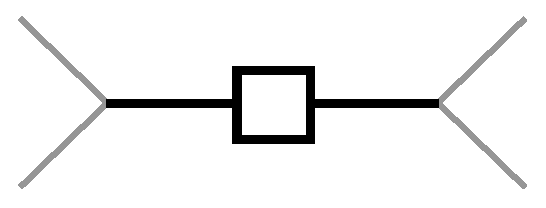
\includegraphics[scale = 0.4]{images/process}
  \caption{The \PD glyph for \glyph{process}.}
  \label{fig:process}
\end{figure}

A process is the basic process node in SBGN.  It describes a process that transforms a given set of biochemical entities---macromolecules, simple chemicals or unspecified entities---into another set of biochemical entities.  Such a transformation might imply modification of covalent bonds (conversion), modification of the relative position of constituents (conformational process) or movement from one compartment to another (translocation).

A cardinality label may be associated with \glyph{consumption} (\sect{consumption}) or \glyph{production} (\sect{production}) arcs to indicate the stoichiometry of the process.  This label becomes a requirement when the exact composition of the number of copies of the inputs or outputs to a reaction are ambiguous in the map.

A process is regarded as reversible if both `sides' of the process are connected to \glyph{production} arcs (see section \ref{sec: semantics reversible procs}).

The example in \fig{trans-phos} illustrates the use of a \glyph{process} node to represent the phosphorylation of a protein in a \PD.

\begin{figure}[H]
  \centering
  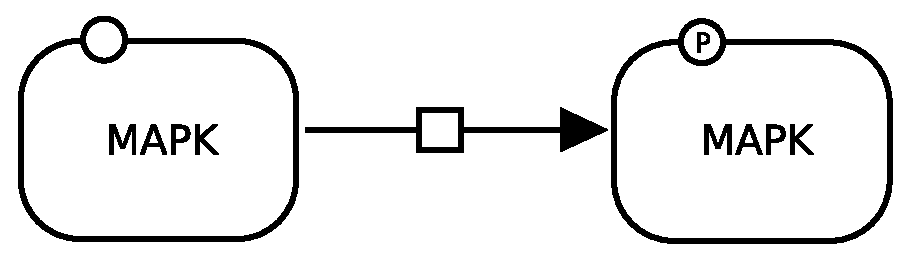
\includegraphics[scale = 0.3]{examples/process-phosphorylation}
  \caption{Phosphorylation of the protein MAP kinase.}
  \label{fig:trans-phos}
\end{figure}

The example in \fig{trans-react} illustrates the use of a \glyph{process} node to represent a reaction between two reactants that generates three products. 

\begin{figure}[H]
  \centering
  \includegraphics[scale = 0.3]{examples/process-reaction}
  \caption{Reaction between ATP and fructose-6-phosphate to produce fructose-1,6-biphosphate, ADP and a proton.}
  \label{fig:trans-react}
\end{figure}

The example in \fig{trans-trans} illustrates the use of a \glyph{process} node to represent a translocation. The large round-cornered rectangle represents a compartment border (see \sect{compartment}).

\begin{figure}[H]
  \centering
  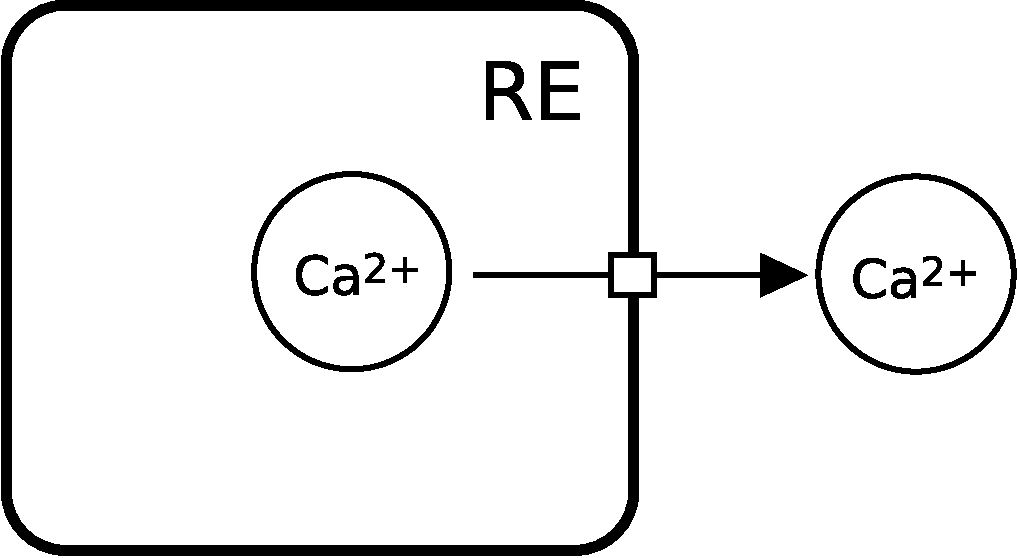
\includegraphics[scale = 0.3]{examples/process-translocation}
  \caption{Translocation of calcium ion out of the endoplasmic reticulum. Note that the \glyph{process} does not have to be located on the boundary of the \glyph{compartment}. A \glyph{process} is not attached to any \glyph{compartment}.}
  \label{fig:trans-trans}
\end{figure}

The example in \fig{trans-reverse} illustrates the use of a \glyph{process} node to represent the reversible opening and closing of an ionic channel in a \PD.

\begin{figure}[H]
  \centering
  \includegraphics[scale = 0.3]{examples/process-reversible}
  \caption{Reversible opening and closing of an ionic channel.}
  \label{fig:trans-reverse}
\end{figure}

When such a reversible process is asymmetrically modulated, it must be represented by two different processes in a \PD.  \fig{trans-mod} illustrates the use of two \glyph{process} nodes to represent the reversible activation of a G-protein coupled receptor.  In the absence of any effector, an equilibrium exists between the inactive and active forms.  The agonist stabilises the active form, while the inverse agonist stabilises the inactive form.

\begin{figure}[H]
  \centering
  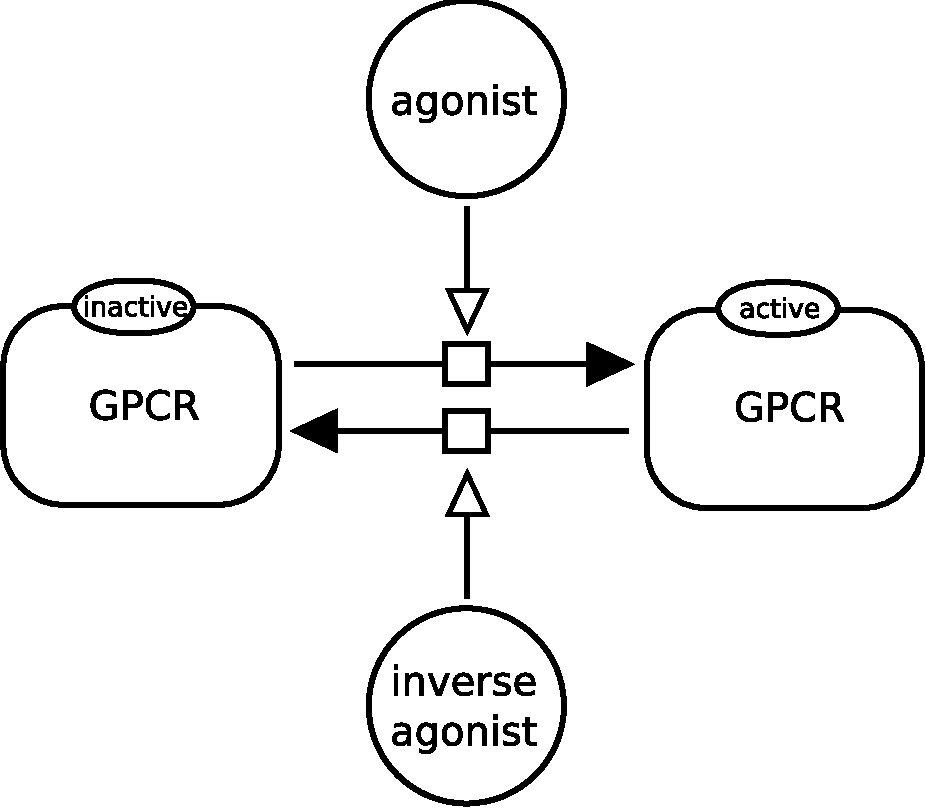
\includegraphics[scale = 0.3]{examples/process-modulated}
  \caption{The reversible activation of a G-protein coupled receptor.}
  \label{fig:trans-mod}
\end{figure}

The example in \fig{trans-dim} presents the conversion of two galactoses into a lactose.  Galactoses are represented by only one \glyph{simple chemical}, the cardinality being carried by the \glyph{consumption} arc.

\begin{figure}[H]
  \centering
  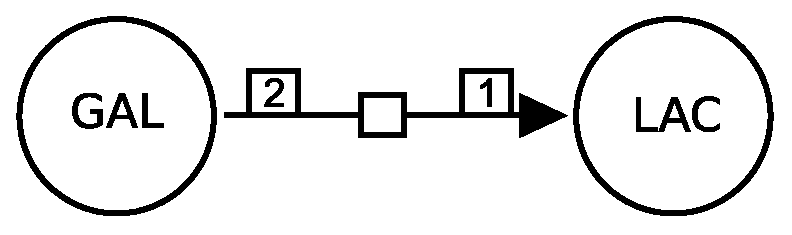
\includegraphics[scale = 0.3]{examples/process-dimerisation}
  \caption{Conversion of two galactoses into a lactose.}
  \label{fig:trans-dim}
\end{figure}




% The following is for [X]Emacs users.  Please leave in place.
% Local Variables:
% TeX-master: "../sbgn_PD-level1"
% End:
